\documentclass{article}
\usepackage{import}
\import{../../../lib/latex/}{wgmlgz}

\begin{document}

\itmo[
       variant=112,
       labn=1,
       worktype=Курсовая работа часть,
       discipline=Дискретная математика,
       group=P3115,
       student=Владимир Мацюк,
       teacher=Поляков Владимир Иванович,
       logo=../../../lib/img/itmo.png
]

\newcommand{\car}{\multicolumn{1}{c@{\hspace*{\tabcolsep}\makebox[0pt]{\curvearrowleft}}}{}}
\newcommand{\rcar}{\multicolumn{1}{c@{\hspace*{\tabcolsep}\makebox[0pt]{\curvearrowright}}}{}}
\newcommand{\ncar}{\multicolumn{1}{c@{\hspace*{\tabcolsep}\makebox[0pt]{}}}{}}
\newcommand{\SPACE}{\multicolumn{12}{c}{}}
\newcommand{\INT}{\multicolumn{5}{c}{\MM{Интерпретации}}}
\newcommand{\PLUS}{\multirow{2}{*}{+}}
\newcommand{\MINUS}{\multirow{2}{*}{-}}
\newcommand{\SIGN}{\multicolumn{2}{c}{\MM{Знаковая}}}
\newcommand{\USIGN}{\multicolumn{2}{c}{\MM{Беззнаковая}}}

\section{Вариант}
$$
       \begin{tabular}{|c|c|}
              \hline
              Условия, при которых $f=1$ & $3 \le |x_4 1 x_5 - x_1x_2x_3| < 6$ \nl
              Условия, при которых $f=d$ & $|x_4 1 x_5 - x_1x_2x_3| = 0$ \nl
       \end{tabular}
$$
\section{Задание}

\begin{enumerate}
       \item Составить таблицу истинности заданной булевой функции.
             $$\begin{array}{|c|c|c|c|c|c|c|c|c|c|c|} \hline
                           N  & x_1x_2x_3x_4x_5 & x_41x_5 & (x_41x_5)_{10} & x_1x_2x_3 & (x_1x_2x_3)_{10} & |x_4 1 x_5 - x_1x_2x_3| & f \nl
                           0  & 00000           & 010     & 2              & 000       & 0                & 2                       & 0 \nl
                           1  & 00001           & 011     & 3              & 000       & 0                & 3                       & 1 \nl
                           2  & 00010           & 110     & 6              & 000       & 0                & 6                       & 0 \nl
                           3  & 00011           & 111     & 7              & 000       & 0                & 7                       & 0 \nl
                           4  & 00100           & 010     & 2              & 001       & 1                & 1                       & 0 \nl
                           5  & 00101           & 011     & 3              & 001       & 1                & 2                       & 0 \nl
                           6  & 00110           & 110     & 6              & 001       & 1                & 5                       & 1 \nl
                           7  & 00111           & 111     & 7              & 001       & 1                & 6                       & 0 \nl
                           8  & 01000           & 010     & 2              & 010       & 2                & 0                       & d \nl
                           9  & 01001           & 011     & 3              & 010       & 2                & 1                       & 0 \nl
                           10 & 01010           & 110     & 6              & 010       & 2                & 4                       & 1 \nl
                           11 & 01011           & 111     & 7              & 010       & 2                & 5                       & 1 \nl
                           12 & 01100           & 010     & 2              & 011       & 3                & 1                       & 0 \nl
                           13 & 01101           & 011     & 3              & 011       & 3                & 0                       & d \nl
                           14 & 01110           & 110     & 6              & 011       & 3                & 3                       & 1 \nl
                           15 & 01111           & 111     & 7              & 011       & 3                & 4                       & 1 \nl
                           16 & 10000           & 010     & 2              & 100       & 4                & 2                       & 0 \nl
                           17 & 10001           & 011     & 3              & 100       & 4                & 1                       & 0 \nl
                           18 & 10010           & 110     & 6              & 100       & 4                & 2                       & 0 \nl
                           19 & 10011           & 111     & 7              & 100       & 4                & 3                       & 1 \nl
                           20 & 10100           & 010     & 2              & 101       & 5                & 3                       & 1 \nl
                           21 & 10101           & 011     & 3              & 101       & 5                & 2                       & 0 \nl
                           22 & 10110           & 110     & 6              & 101       & 5                & 1                       & 0 \nl
                           23 & 10111           & 111     & 7              & 101       & 5                & 2                       & 0 \nl
                           24 & 11000           & 010     & 2              & 110       & 6                & 4                       & 1 \nl
                           25 & 11001           & 011     & 3              & 110       & 6                & 3                       & 1 \nl
                           26 & 11010           & 110     & 6              & 110       & 6                & 0                       & d \nl
                           27 & 11011           & 111     & 7              & 110       & 6                & 1                       & 0 \nl
                           28 & 11100           & 010     & 2              & 111       & 7                & 5                       & 1 \nl
                           29 & 11101           & 011     & 3              & 111       & 7                & 4                       & 1 \nl
                           30 & 11110           & 110     & 6              & 111       & 7                & 1                       & 0 \nl
                           31 & 11111           & 111     & 7              & 111       & 7                & 0                       & d \nl
                    \end{array}$$
             
       \item Представить булеву функцию в аналитическом виде с помощью КДНФ и ККНФ.
             \begin{itemize}
                    \item КДНФ: $(\bar{x}_1∧\bar{x}_2∧\bar{x}_3∧\bar{x}_4∧x_5) ∨ (\bar{x}_1∧\bar{x}_2∧x_3∧x_4∧\bar{x}_5) ∨ (\bar{x}_1∧x_2∧\bar{x}_3∧x_4∧\bar{x}_5) ∨ (\bar{x}_1∧x_2∧\bar{x}_3∧x_4∧x_5) ∨ (\bar{x}_1∧x_2∧x_3∧x_4∧\bar{x}_5) ∨ (\bar{x}_1∧x_2∧x_3∧x_4∧x_5) ∨ (x_1∧\bar{x}_2∧\bar{x}_3∧x_4∧x_5) ∨ (x_1∧\bar{x}_2∧x_3∧\bar{x}_4∧\bar{x}_5) ∨ (x_1∧x_2∧\bar{x}_3∧\bar{x}_4∧\bar{x}_5) ∨ (x_1∧x_2∧\bar{x}_3∧\bar{x}_4∧x_5) ∨ (x_1∧x_2∧x_3∧\bar{x}_4∧\bar{x}_5) ∨ (x_1∧x_2∧x_3∧\bar{x}_4∧x_5)$
                    \item ККНФ: $(x_1∨x_2∨x_3∨x_4∨x_5) ∧ (x_1∨x_2∨x_3∨\bar{x}_4∨x_5) ∧ (x_1∨x_2∨x_3∨\bar{x}_4∨\bar{x}_5) ∧ (x_1∨x_2∨\bar{x}_3∨x_4∨x_5) ∧ (x_1∨x_2∨\bar{x}_3∨x_4∨\bar{x}_5) ∧ (x_1∨x_2∨\bar{x}_3∨\bar{x}_4∨\bar{x}_5) ∧ (x_1∨\bar{x}_2∨x_3∨x_4∨\bar{x}_5) ∧ (x_1∨\bar{x}_2∨\bar{x}_3∨x_4∨x_5) ∧ (\bar{x}_1∨x_2∨x_3∨x_4∨x_5) ∧ (\bar{x}_1∨x_2∨x_3∨x_4∨\bar{x}_5) ∧ (\bar{x}_1∨x_2∨x_3∨\bar{x}_4∨x_5) ∧ (\bar{x}_1∨x_2∨\bar{x}_3∨x_4∨\bar{x}_5) ∧ (\bar{x}_1∨x_2∨\bar{x}_3∨\bar{x}_4∨x_5) ∧ (\bar{x}_1∨x_2∨\bar{x}_3∨\bar{x}_4∨\bar{x}_5) ∧ (\bar{x}_1∨\bar{x}_2∨x_3∨\bar{x}_4∨\bar{x}_5) ∧ (\bar{x}_1∨\bar{x}_2∨\bar{x}_3∨\bar{x}_4∨x_5) $
             \end{itemize}
       \item Найти МДНФ и/или МКНФ методом Квайна – Мак-Класки.
             $$\begin{array}{|l|l|l|l|l|l|l|l|l|l|l|l|l|l|l|l|l|l|} \hline
                           \textnumero & K^0   &   & \textnumero & K^1   &       &   & \textnumero & K^2   &       & \textnumero & Z(f) \nl
                           1           & 00001 &   & 1           & 0x110 & 2-7   &   & 1           & x10x0 & 2-14  & 1           & 00001 \nl
                           2           & 00110 & ✓ & 2           & 010x0 & 3-4   & ✓ & 2           & 01x1x & 4-10  & 2           & 10011 \nl
                           3           & 01000 & ✓ & 3           & x1000 & 3-11  & ✓ & 3           & x11x1 & 8-18  & 3           & 0x110 \nl
                           4           & 01010 & ✓ & 4           & 0101x & 4-5   & ✓ & 4           & 11x0x & 13-17 & 4           & 1x100 \nl
                           5           & 01011 & ✓ & 5           & 01x10 & 4-7   & ✓ &             &       &       & 5           & x10x0 \nl
                           6           & 01101 & ✓ & 6           & x1010 & 4-13  & ✓ &             &       &       & 6           & 01x1x \nl
                           7           & 01110 & ✓ & 7           & 01x11 & 5-8   & ✓ &             &       &       & 7           & x11x1 \nl
                           8           & 1111  & ✓ & 8           & 011x1 & 6-8   & ✓ &             &       &       & 8           & 11x0x \nl
                           9           & 10011 &   & 9           & x1101 & 6-15  & ✓ &             &       &       &             & \nl
                           10          & 10100 & ✓ & 10          & 0111x & 7-8   & ✓ &             &       &       &             & \nl
                           11          & 11000 & ✓ & 11          & x1111 & 8-16  & ✓ &             &       &       &             & \nl
                           12          & 11001 & ✓ & 12          & 1x100 & 10-14 &   &             &       &       &             & \nl
                           13          & 11010 & ✓ & 13          & 1100x & 11-12 & ✓ &             &       &       &             & \nl
                           14          & 11100 & ✓ & 14          & 110x0 & 11-13 & ✓ &             &       &       &             & \nl
                           15          & 11101 & ✓ & 15          & 11x00 & 11-14 & ✓ &             &       &       &             & \nl
                           16          & 11111 & ✓ & 16          & 11x01 & 12-15 & ✓ &             &       &       &             & \nl
                                       &       &   & 17          & 1110x & 14-15 & ✓ &             &       &       &             & \nl   
                                       &       &   & 18          & 111x1 & 15-16 & ✓ &             &       &       &             & \nl   
                    \end{array}$$
             Импликантная таблица:
             \begin{center}
                    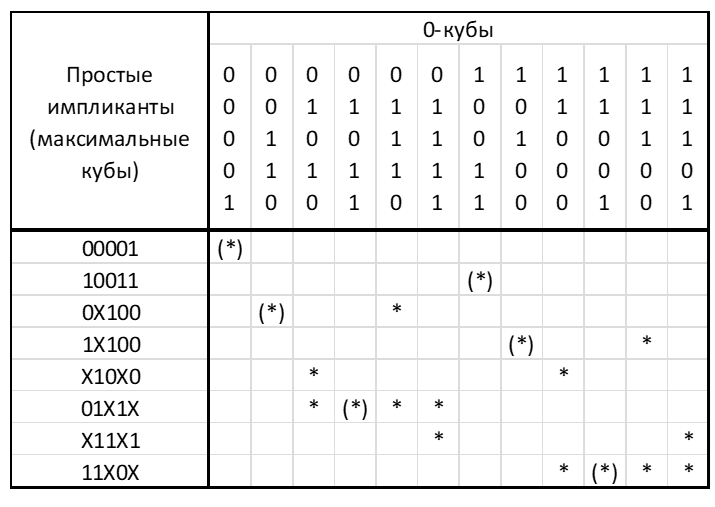
\includegraphics[scale=0.5]{img1.png}
             \end{center}
             
             Ядро покрытия:
             
             $$T =\left\{\begin{array}{c}
                           00001 \\
                           0x110 \\
                           1x100 \\
                           01x1x \\
                           11x0x \\
                           10011
                    \end{array}\right\},\ C_{min} (f)=\left\{\begin{array}{c}
                           00001 \\
                           0x110 \\
                           1x100 \\
                           01x1x \\
                           11x0x \\
                           10011
                    \end{array}\right\}$$
             $$S_a = 24,\ S_b= 30$$
             $$f = (x_1x_2\bar{x}_4) ∨ (\bar{x}_1x_2x_4) ∨ (x_1x_3\bar{x}_4\bar{x}_5) ∨ (\bar{x}_1x_3x_4\bar{x}_5) ∨ (x_1\bar{x}_2\bar{x}_3x_4x_5) ∨ (\bar{x}_1\bar{x}_2\bar{x}_3\bar{x}_4x_5)$$
       \item Найти МДНФ и МКНФ на картах Карно.
             $$\begin{array}{|c|c|c|c|c|c|c|c|c|c|c|c|c|c|} \hline
                           $\backslashbox{$x_1x_2$}{$x_3x_4x_5$}$ & 000 & 001 & 011 & 010 & 110 & 111 & 101 & 100 \nl
                           00                                     & 0   & 1   & 0   & 0   & 1   & 0   & 0   & 0 \nl
                           01                                     & d   & 0   & 1   & 1   & 1   & 1   & d   & 0 \nl
                           11                                     & 1   & 1   & 0   & d   & 0   & d   & 1   & 1 \nl
                           10                                     & 0   & 0   & 1   & 0   & 0   & 0   & 0   & 1 \nl
                           
                    \end{array} $$
             Минимизированная ДНФ:
             $$f = (x_1x_2\bar{x}_4) ∨ (\bar{x}_1x_2x_4) ∨ (x_1x_3\bar{x}_4\bar{x}_5) ∨ (\bar{x}_1x_3x_4\bar{x}_5) ∨ (x_1\bar{x}_2\bar{x}_3x_4x_5) ∨ (\bar{x}_1\bar{x}_2\bar{x}_3\bar{x}_4x_5)$$
             $$S_a = 24,\ S_b= 30$$
             Минимизированная КНФ:
             $$ f = (\bar{x}_2∨\bar{x}_3∨\bar{x}_5) ∧ (\bar{x}_1∨\bar{x}_2∨x_4∨x_5) ∧ (x_1∨\bar{x}_2∨\bar{x}_4∨x_5) ∧  (x_1∨x_2 ∨x_4) ∧  (\bar{x}_1∨x_2 ∨\bar{x}_4)  ∧ (\bar{x}_1∨x_3∨\bar{x}_4) ∧ (x_1∨x_3∨x_4)$$
             $$ S_a = 23,\ S_b= 30$$
       \item Преобразовать МДНФ и МКНФ к форме, обеспечивающей минимум цены схемы.
             \begin{itemize}
                    \item Факторное преобразование для МДНФ:
                          $$ (x_1x_2\bar{x}_4) ∨ (\bar{x}_1x_2x_4) ∨ (x_1x_3\bar{x}_4\bar{x}_5) ∨ (\bar{x}_1x_3x_4\bar{x}_5) ∨ (x_1\bar{x}_2\bar{x}_3x_4x_5) ∨ (\bar{x}_1\bar{x}_2\bar{x}_3\bar{x}_4x_5) =
                          $$ $$ =(x_2 (x_1\bar{x}_4 ∨ \bar{x}_1x_4)) ∨ (x_3\bar{x}_5(x_1\bar{x}_4 ∨ \bar{x}_1x_4)) ∨ (\bar{x}_2\bar{x}_3x_5 (x_1x_4 ∨ \bar{x}_1\bar{x}_4)) $$
                          $$ φ= x_1\bar{x}_4 ∨ \bar{x}_1x_4 $$
                          $$ (x_2φ) ∨ (x_3\bar{x}_5φ) ∨ (\bar{x}_2\bar{x}_3x_5¬φ) $$
                          $$ S_Q^F= 13,\ S_Q^φ = 7$$
                    \item Факторное преобразование для МКНФ:
                          $$ (\bar{x}_2∨\bar{x}_3∨\bar{x}_5) ∧ (\bar{x}_1∨\bar{x}_2∨x_4∨x_5) ∧ (x_1∨\bar{x}_2∨\bar{x}_4∨x_5) ∧  (x_1∨x_2 ∨x_4) ∧  (\bar{x}_1∨x_2 ∨\bar{x}_4)  ∧ (\bar{x}_1∨x_3∨\bar{x}_4) ∧ (x_1∨x_3∨x_4) = $$
                          $$          = (\bar{x}_2∨\bar{x}_3∨\bar{x}_5) ∧ (\bar{x}_2∨x_5∨((\bar{x}_1∨x_4) ∧ (x_1∨\bar{x}_4))) ∧  (x_2 ∨ ((x_1∨x_4) ∧  (\bar{x}_1 ∨\bar{x}_4)))  ∧ (x_3∨(\bar{x}_1∨ \bar{x}_4) ∧ (x_1∨x_4)) $$
                          $$φ= (x_1∨x_4) ∧  (\bar{x}_1 ∨\bar{x}_4) $$
                          $$ = (\bar{x}_2∨\bar{x}_3∨\bar{x}_5) ∧ (\bar{x}_2∨x_5∨¬ φ) ∧  (x_2 ∨ φ)  ∧ (x_3∨ φ)=	$$
                          $$ S_Q^F= 15,\ S_Q^φ = 7$$
             \end{itemize}
             
       \item По полученной форме построить комбинационную схему в булевом базисе. Определить задержку схемы.
             $$ S_Q  = 20,\ τ=5t $$
             \begin{center}
                    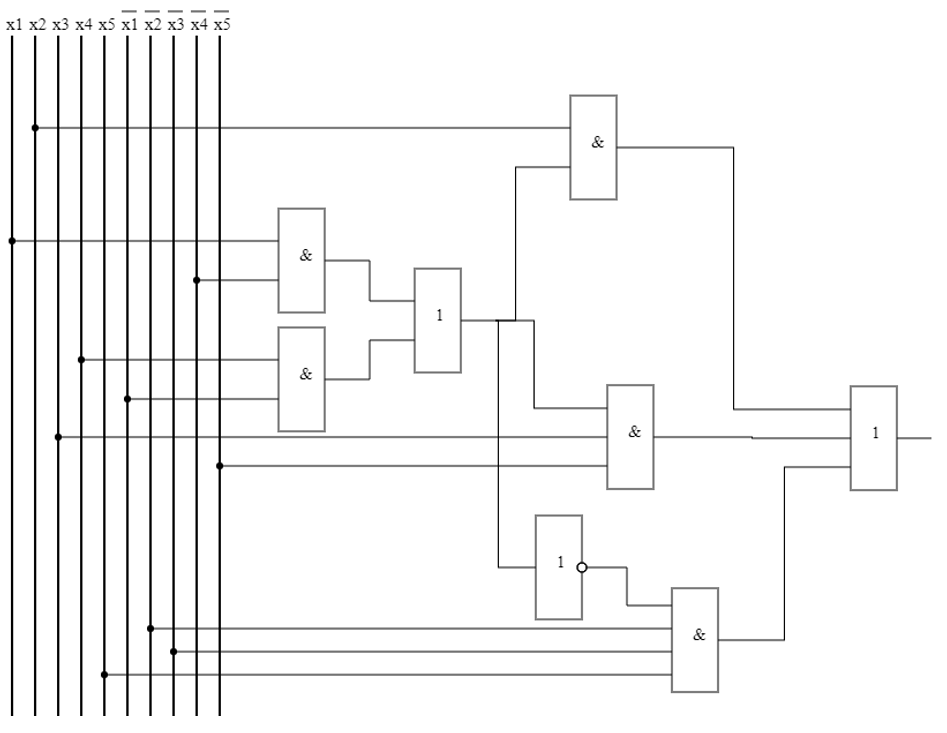
\includegraphics[scale=0.4]{img2.png}
             \end{center}
       \item Построить схемы с минимальной ценой в универсальных базисах и сокращенных булевых базисах. Определить задержку каждой из схем.
             Синтез комбинационных схем в универсальных базисах
             % Базис (И-НЕ)
             % φ= x_1\bar{x}_4 ∨ \bar{x}_1x_4 = ¬¬(x_1\bar{x}_4 ∨ \bar{x}_1x_4) = ¬(¬(x_1∧\bar{x}_4) ∧ ¬ (\bar{x}_1∧x_4)) =
             % = (x_1 |\bar{x}_4) | (\bar{x}_1 | x_4)
             % f =(x_2φ) ∨ (x_3\bar{x}_5φ) ∨ (\bar{x}_2\bar{x}_3x_5(x_1x_4 ∨ \bar{x}_1\bar{x}_4))=
             % =(x_2|φ) | (x_3|\bar{x}_5|φ) | (\bar{x}_2|\bar{x}_3|x_5|((x_1|x_4)| (\bar{x}_1|\bar{x}_4)))
             % SQ F= 18, 	SQ φ = 7
             % SQ  = 25, 	τ=4t
             
       \item Построить схему в базисе Жегалкина. Определить цену и задержку.
       \item Построить схему в универсальном базисе с учетом заданного коэффициента объединения по входам. Определить цену и задержку схемы.
       \item Выполнить анализ построенных схем, определив их реакцию на заданные комбинации входных сигналов.
\end{enumerate}
\section{Решение}
\end{document}
